\problema{(Rod�zio de Pizza)}

\begin{descricao}
O os alunos do curso comunit�rio de culin�ria ``Experimentando Receitas Italianas'' tiveram uma ideia para aproveitar os pratos feitos no curso: ser� feito um evento beneficente para crian�as carentes. Para isso, ser�o feitas pizzas para serem servidas no evento. As pizzas ser�o cortadas em 8 fatias id�nticas e servidas em pratos do pr�prio curso. Entretanto, as pizzas de diferentes alunos s�o de diferentes tamanhos. Al�m disso, o pratos do curso s�o oriundos de doa��es, tendo-se assim diversos modelos distintos. Por raz�es de higiene, uma fatia s� pode ser servida em um prato se ela couber completamente naquele prato. Como a quantidade de pizzas ser� grande, voc� foi contratado para desenvolver um programa que, a partir de uma lista contendo raio de cada pizza e os raios dos pratos, diga qual a maior quantidade de pizzas que pode ser servida de maneira adequada.
\begin{center}
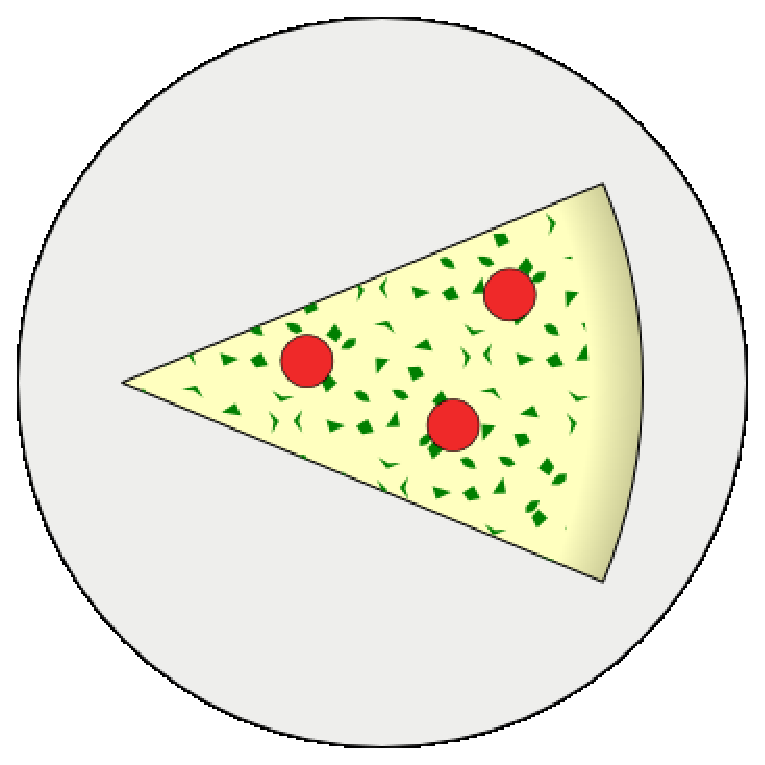
\includegraphics[scale=0.4]{pizza/pizza.eps}
\end{center}

\end{descricao}

\begin{entrada}
A entrada � composta por diversas inst�ncias do problema. Cada inst�ncia � composta por 3 linhas. A primeira linha cont�m 2 n�meros inteiros, $m$ e $n$, $1 \leq m \leq 1000000$, $1 \leq n \leq 1000000$ as quantidades de pizzas e pratos, respectivamente. A segunda linha cont�m m n�meros inteiros, indicando os raios das pizzas. A terceira linha cont�m n n�meros inteiros, contendo os tamanhos dos pratos. A entrada termina quando $m=n=0$. Essa inst�ncia n�o deve ser processada.
\end{entrada}

\begin{saida}
Para cada inst�ncia de entrada deve ser impresso uma �nica linha contendo um inteiro referente � quantidade de fatias de pizza que podem ser servidas de maneira adequada.
\end{saida}

\exemplos{0.47}{0.47}
{2 10			\pl
5 5			\pl
3 3 5 5 5 5 5 5 5 5	\pl
2 10			\pl
50 5			\pl
3 3 5 5 5 5 5 5 5 5	\pl
0 0
}
{10	\pl
2
}

%\pb
